
\begin{center}
    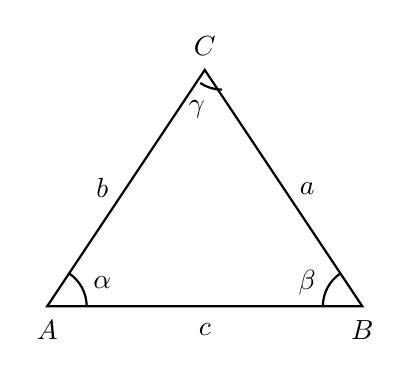
\begin{tikzpicture}
        % Define the points of the triangle
        \coordinate (A) at (0, 0);
        \coordinate (B) at (4, 0);
        \coordinate (C) at (2, 3);
    
        % Draw the sides of the triangle
        \draw[thick] (A) -- (B) -- (C) -- cycle;
    
        % Label the sides
        \node at (2, -0.3) {$c$};
        \node at (3.3, 1.5) {$a$};
        \node at (0.7, 1.5) {$b$};
    
        % Label the angles
        \node at (0, -0.3) {$A$};
        \node at (4, -0.3) {$B$};
        \node at (2, 3.3) {$C$};
    
        % Mark the angles
        \draw[thick] (0.5,0) arc[start angle=0,end angle=56.31,radius=0.5];
        \node at (0.7, 0.3) {$\alpha$};
        
        \draw[thick] (3.5,0) arc[start angle=180,end angle=123.69,radius=0.5];
        \node at (3.3, 0.3) {$\beta$};
        
        \draw[thick] (2.22,2.75) arc[start angle=270,end angle=236.31,radius=0.5];
        \node at (1.9, 2.5) {$\gamma$};
    
    \end{tikzpicture}
    \end{center}


